\begin{figure}[H]
\centering
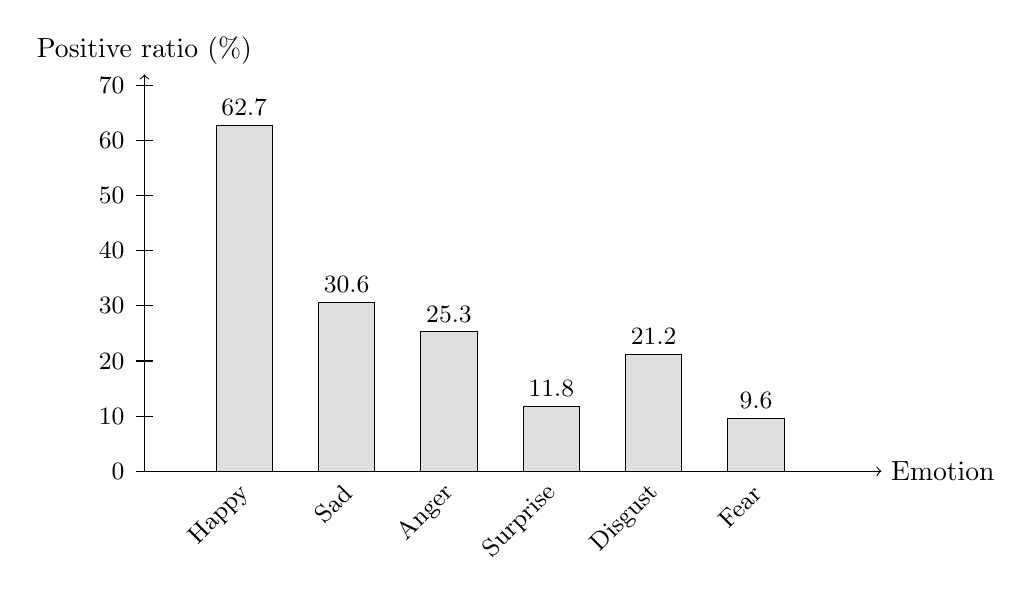
\begin{tikzpicture}[
    x=1.3cm,
    y=0.07cm
]

% Axes
\draw[->] (0,0) -- (7.2,0) node[right] {Emotion};
\draw[->] (0,0) -- (0,72) node[above] {Positive ratio (\%)};

% Y ticks
\foreach \y in {0,10,20,30,40,50,60,70} {
    \draw (-0.08,\y) -- (0.08,\y);
    \node[left] at (-0.1,\y) {\small \y};
}

% Bars: x, height, label
\foreach \x/\h/\name in {
    0.7/62.7/Happy,
    1.7/30.6/Sad,
    2.7/25.3/Anger,
    3.7/11.8/Surprise,
    4.7/21.2/Disgust,
    5.7/9.6/Fear
} {
    \draw[fill=gray!25] (\x,0) rectangle +(0.55,\h);
    \node[above, font=\small] at (\x+0.275,\h) {\h};
    \node[rotate=45, anchor=east, font=\small] at (\x+0.35,-2) {\name};
}

\end{tikzpicture}
\caption{Class imbalance in the filtered CMU-MOSEI six-emotion dataset.}
\label{fig:class_distribution}
\end{figure}